\chapter{The LHC and the CMS detector}
\section{The Large Hadron Collider}
The LHC is a ring-shaped proton-proton accelerator with a circumference of
\unit[27]{km}. It is hosted in a tunnel 45 to \unit[170]{m} below ground at
the CERN laboratory in Geneva, Switzerland. In 2011, the LHC accelerated two
proton beams up to an energy of \unit[3.5]{TeV} each and an instantaneous
luminosity of up to $\unit[3.5\cdot 10^{33}]{cm^{-2}s^{-1}}$.

The two proton beams are pre-accelerated through four smaller systems before
being injected in the LHC:
\begin{itemize}
    \item the linear accelerator (up to \unit[50]{MeV})
    \item the proton synchrotron booster (up to \unit[1.4]{GeV})
    \item the proton synchrotron (up to \unit[26]{GeV})
    \item the super proton synchrotron (up to \unit[450]{GeV})
\end{itemize}

The protons travel in ultra-high vacuum around
$\unit[10^{-10}]{mbar}$, while different sets of magnets keep them in a
circular orbit and provide acceleration and focusing.

Radio frequency cavities in the LHC accelerate the protons, providing an energy
increase of $\unitfrac[0.5]{MeV}{turn}$.
Superconducting dipole magnets operate at currents of \unit[11850]{A} to bend the trajectories
of the protons with a magnetic field up to \unit[8.3]{T}.
Quadrupole magnets are employed to focus the beams, thus increasing the
probability of an interaction when they collide.
The magnets are cooled with superfluid helium at \unit[1.9]{K}.
The beams are made of ``bunches'' of protons with a time spacing of
\unit[75]{ns}.

At four different interaction points, the two proton beams are brought to
collision where the experiments are located: CMS, ATLAS, LHCb and ALICE.
The first two are general purpose detectors. LHCb is designed for the study
of CP violation in $\mathrm{b}$ physics, and ALICE for the analysis of the
quark-gluon plasma produced mainly in heavy ion collisions.

\section{The Compact Muon Solenoid}
CMS is a general purpose detector based on interlocking cylindrical
subdetectors in the central \emph{barrel} region, closed by two
\emph{endcaps}, all placed coaxially with the beam and centred on the beam interaction point.
\subsection{Coordinate convention}
The conventional coordinate system has its origin at the nominal interaction
point. The $z$ axis points along the beam direction, the $y$ axis points
vertically upwards, and the $x$ axis points towards the centre of the LHC
circumference. The $xy$ plane is thus called the \emph{transverse} plane as
it is orthogonal to the CMS cylinder.

We define two angles in the transverse plane: the azimuthal $\varphi$ angle
is measured from the $x$ axis, and the polar angle $\theta$, measured from
the $z$ axis.
\emph{Pseudorapidity} is defined as $\eta = -\log \tan
\nicefrac{\theta}{2}$.

\subsection{Structure of the detector}
A global view and a transverse section of the detector are shown in
figures~\ref{fig:cms} and~\ref{fig:cms_transverse}.

\begin{figure}[htb]
    \centering
    \includegraphics[width=\textwidth]{images/pdf/cms}
    \caption{The CMS detector.}
    \label{fig:cms}
\end{figure}

\begin{figure}[htb]
    \centering
    \includegraphics[width=\textwidth]{images/pdf/cms_transverse}
    \caption{Transverse view of the CMS detector with sample tracks.}
    \label{fig:cms_transverse}
\end{figure}

A superconducting solenoid \unit[13.5]{m} and with a diameter of
\unit[5.9]{m} provides a uniform, axial magnetic field of \unit[3.8]{T}.
The return field saturates an iron yoke, which consists of five wheels in
the barrel region and three disks in each of the two endcaps.
Muon detectors are installed in the return yokes, with four stations of
aluminium drift tubes in the barrel and cathode strip chambers with
resistive plate chambers in the endcap.

The tracking system and the calorimeters are installed inside the solenoid.
The tracker is a cylinder with a diameter of \unit[2.6]{m} with three layers
of pixel detectors, allowing exceptional measurements of the impact parameter
of the particles and secondary vertex reconstruction, and ten layers of
silicon microstrip detectors.
The tracking system is surrounded by the calorimeters, which cover the
region with $|\eta| < 3$. There is an electromagnetic calorimeter (ECAL),
made of lead tungstate crystals and a brass/scintillator hadron calorimeter
(HCAL). A forward calorimeter provides additional coverage up to $|\eta| <
5$.

\subsection{The tracking system}
Very high granularity and time resolutions are needed in the tough
environment of the LHC experiments, with thousands of particles produced
for every interaction. The high spatial resolution is particularly important
in the region close to the primary interaction.

For these reasons, silicon detectors where chosen for the whole tracking
system of the CMS experiment.

\begin{description}
    \item[The pixel detector] is made of three cylinders in the barrel and
        two disks in each of the two endcaps. The spatial resolution on each
        hit is about \unit[10]{\micro m} in $r$-$\varphi$ and about
        \unit[20]{\micro m} in $z$.
    \item[The microstrip detector] is made of concentrical layers in the
        barrel region, divided in two systems: the \emph{tracker inner
        barrel} (TIB) and the \emph{tracker outer barrel} (TOB).

        The TIB has four layers in the region with $\unit[20]{cm} < r <
        \unit[55]{cm}$ and $|z| < \unit[65]{cm}$. The sensors are
        \unit[10]{cm} long in $z$, 80 to \unit[120]{\micro m} wide and
        \unit[320]{\micro m} thick. The single hit resolution is between 23
        and \unit[34]{\micro m} in the $r$-$\varphi$ plane, and about
        \unit[230]{\micro m} in $z$.

        The TOB module is made of six layers, covering
        $\unit[55]{cm} < r < \unit[116]{cm}$ and $|z| <
        \unit[116]{cm}$. The sensors have a length of \unit[25]{cm}, a width
        of \unit[180]{\micro m} and a thickness of \unit[500]{\micro m}. The
        single hit resolution is 35 to \unit[52]{\micro m} in the
        $r$-$\varphi$ coordinates, and \unit[530]{\micro m} in $z$.

        Two more modules are installed in the endcaps, arranged around the
        beam line: the \emph{tracker inner
        disks} (TID) and \emph{tracker outer endcaps} (TEC)

        Each TEC module consists of nine disks, while the TID have three
        smaller disks. Both these modules have strips pointing radially
        toward the beam line with a thickness of \unit[320]{\micro m} to
        \unit[500 \micro]{m}.
\end{description}

\subsection{The electromagnetic calorimeter}
The ECAL is the inner calorimeter, made of 61200 lead tungstate crystals in
the barrel and 7324 crystals in the endcaps.
The base of the crystals is about $\unit[2\times2]{cm}$ in size, with a
depth of $\unit[23]{cm}$, corresponding to 25 radiation lengths.

The scintillation light is collected by avalanche photodiodes in the barrel
and vacuum phototriodes in the endcaps. They have a high gain and are
insensitive to the magnetic field of the detector.

The energy resolution of the calorimeter has been measured in $\Z
\rightarrow \E\E$ events from the 2011 data~\cite{CMS-DP-2012-007}, as shown in
figure~\ref{fig:ecal_resolution}.

\begin{figure}[htb]
    \centering
    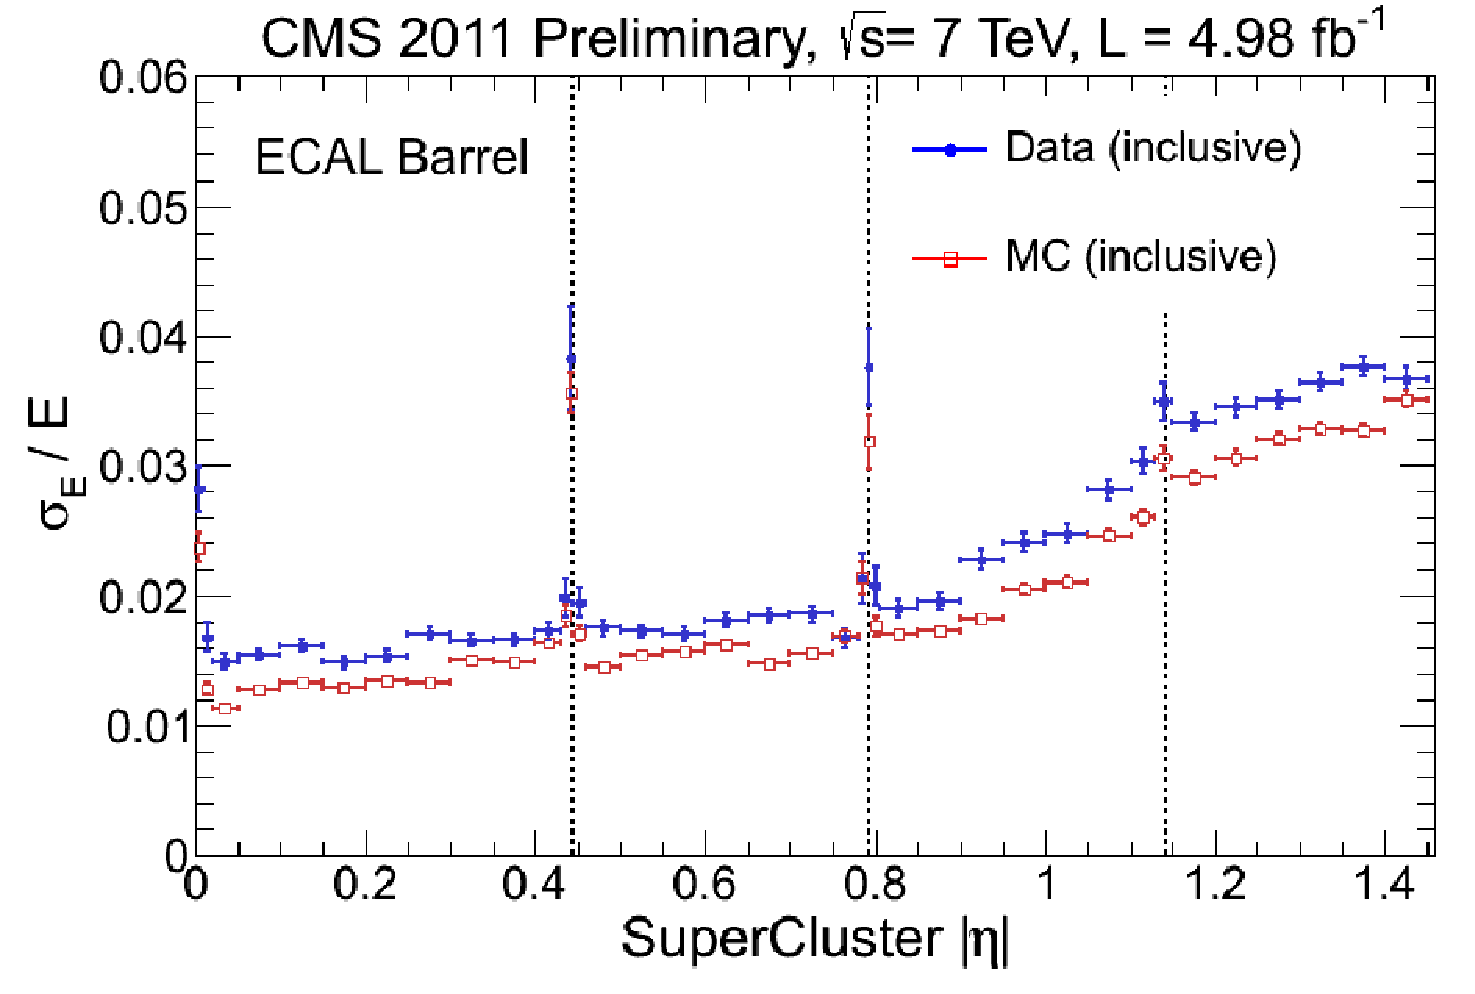
\includegraphics[width=.48\textwidth]{images/pdf/ecal_barrel_resolution}
    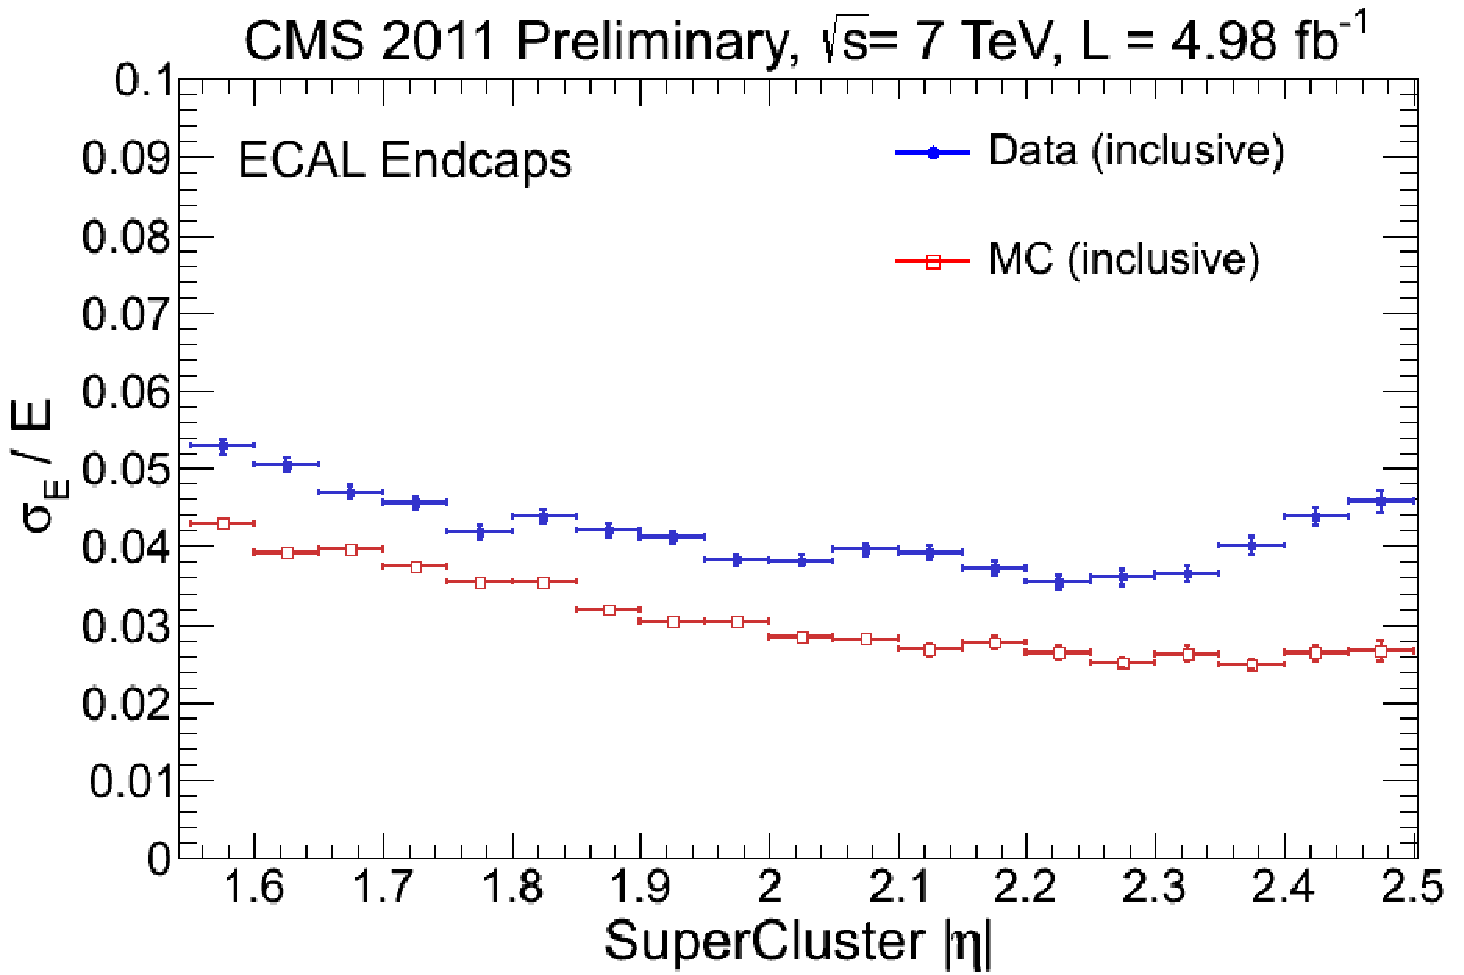
\includegraphics[width=.48\textwidth]{images/pdf/ecal_endcap_resolution}
    \caption{Energy resolution of the ECAL as measured in $\Z \rightarrow
    \E\E$ events in the 2011 data.}
    \label{fig:ecal_resolution}
\end{figure}

\subsection{The hadron calorimeter}
The HCAL surrounds the ECAL and is made of plastic scintillators interleaved with brass layers.
